\documentclass[11pt]{report}

%%%%%%%%%%%%%%%%%%%%%%%%%%%%%%%%%%%%%%%%%%%%%%%%%%%%%%%%%%%%%%%%%%%%%%
% Theoretical Grounds And Market Adaptations of Financial Fx Options
%%%%%%%%%%%%%%%%%%%%%%%%%%%%%%%%%%%%%%%%%%%%%%%%%%%%%%%%%%%%%%%%%%%%%%

% Packages to use
\usepackage{amsmath}
\usepackage{amssymb}
\usepackage[T1]{fontenc} %uncomment to display chapters
\usepackage{titlesec, color}
\usepackage[numbers]{natbib}
\bibliographystyle{plainnat}
\usepackage{array}
\usepackage{csquotes}
\usepackage{url} % insert Urls in bib
\usepackage{tikz} % images
\usepackage{pgfplots} %images
\usepgfplotslibrary{groupplots}
\usepackage{standalone} % Load tikz from library 
\usepackage{mathrsfs} %Pretty fonts
\usepackage{enumerate} %Roman numerals
\usepackage{amsmath}
\usepackage{amssymb}
\usepackage{amsfonts}
\usepackage{amsthm} % For proofs
\usepackage{mathtools} % For arrows with limits underneath
\usepackage[toc,page]{appendix} %For appendices
\usepackage{bbm} % For indicator functions

%% Defining mathematical environments
\newtheorem{definition}{Definition}[chapter]
\newtheorem{remark}{Remark}[chapter]
\newtheorem{theorem}{Theorem}
\newtheorem{proposition}{Proposition}[chapter]
\newtheorem{corollary}{Corollary}[chapter]


%%%% COMMANDS %%%%
% Real Numbers
\newcommand{\RNums}{\mathbb{R}}
% sigma-algebra
\newcommand{\salg}{\sigma\text{-algebra}}
% borel sigma-algebra
\newcommand{\borelsalg}{\mathscr{B}(\RNums)}
% Indicator function
\newcommand{\ind}{\mathbbm{1}}
% F: Sigma Algebra
\newcommand{\salgF}{\mathscr{F}}
% Probability P
\newcommand{\Pm}{\mathbb{P}}
% Insert only one number in the "align" environment
\newcommand\numberthis{\addtocounter{equation}{1}\tag{\theequation}}


% Document properties
\title{Theoretical Grounds and Market Adaptations of Financial Fx and Interest Rate Options}
\author{Gerardo Dur\'an Mart\'in}

% Command: Chapter Style
\definecolor{gray75}{gray}{0.75}
\newcommand{\hsp}{\hspace{20pt}}
\titleformat{\chapter}[hang]{\Huge\bfseries}{\thechapter\hsp\textcolor{gray75}{|}\hsp}{0pt}{\Huge\bfseries}

% Cite authors. Use \citeauhor*{auth}

% Set line breaks inside cells
\newcommand{\breakcell}[2][c]{%
  \begin{tabular}[#1]{@{}c@{}}#2\end{tabular}}

% Cite as: AUTHOR(YEAR) style
\newcommand{\aycite}[1]{%
 \citeauthor{#1} (\citeyear{#1})}
 
% .............. It starts here ..............
\begin{document}
\tableofcontents

\chapter{Financial Markets}
% TODO: set context: why is it true that te value of something has been of great importance?

Throughout modern history, the value of \textit{anything} has been of great importance. For any two members taking opposite sides of a desired object\footnote{In other words, one member wants to buy (obtain) and the other member to sell (get rid off)}, an exchange takes place if they both agree on the current worth of the object to exchange. For this to happen, both members must be able to find one another. It may also be the case for any of them two to find a third whose worth of the object at play favors any one of them more.\\

A \textbf{security}, is the epitome of a tradable object in financial markets. We define a security as an instrument that either represents ownership or that derives its value from a commodity. We say that a security is \textbf{fungible} if any unit of the instrument is economically indistinguishable from all other units. That is, whomever buys (or sells) the instrument can pay (or receive) any unit at the same price at a given point in time.\\

The problem of searching for the price and the party whose view on the value of a security reflect ours is called \textbf{trading}. A \textbf{market} is the place where buyers meet sellers. Markets can be both a physical place (called a trading floor), or an electronic system.\\

Not all financial products are traded in formal markets. Over the counter (OTC) trades happen between two parties directly or via a broker, whom helps them settle the trade. 

\section{The Participants}
In a financial market, participants have various reasons to trade. On the one hand there is the \textbf{buy-side}. They trade in order to solve a financial problem originated outside of the market. This group sees the market as a means to an end, and thus, they rely on the resources available in the market.\\

\begin{table}[!h]
	\centering
	\begin{tabular}{ c c m{3cm} c}
		\hline
		Trader Type & Examples & Why They Trade & Instruments\\
		\hline
		Investor & \breakcell{Individual \\ Corporate pension funds \\ Insurance funds \\ Charitable and legal trusts \\ Endowments \\ Mutual Funds \\ Money Managers} & {To move wealth from the present to the future for themselves or for their clients} & \breakcell{Stocks \\ Bonds} \\
		\\
		Borrowers & \breakcell{Homeowners \\ Students \\ Corporations} & {To move wealth from the future to the present} & \breakcell{Mortgages \\ Bonds \\ Notes}\\
		\\
		Hedgers & \breakcell{Farmers \\ Manufacturers \\ Miners \\ Shippers \\ Financial Institutions} & {To reduce business operating risk} & \breakcell{Futures contracts \\ Forward contracts \\ Swaps}\\
		\\
		\breakcell{Asset \\ Exchangers} & \breakcell{International corporations \\ Manufacturers \\ Travelers} & {To acquire an asset that they value mire than the asset that they tender} & \breakcell{Currencies \\ Commodities} \\
		\\
		Gamblers & Individuals & {To entertain themselves} & Various\\
		\hline
	\end{tabular}
	\caption{Buy-side of the market. \aycite{harris}}
\end{table}

%
 On the other hand are the participants who offer exchange services to the buy-side. Their trading purpose is to satisfy the needs of the buy-side by taking the opposite side of the trade. This group sells exchange services to the buy-side, consequently they are known as the \textbf{sell-side}.\\

\begin{table}[h!]
    \centering
    \begin{tabular}{c c m{3cm}}
    	\hline
    	Trader Type & Examples & Why They Trade \\
    	\hline
    	Dealer & \breakcell{Market Maker \\ Specialist \\ Floor Trader \\ Locals \\ Day traders \\ Scalpers} & {To earn trading profits by supplying liquidity} \\
    	\\  	
    	Brokers & \breakcell{Retail brokers \\ Discount brokers \\ Full-service brokers \\ Institutional Brokers \\ Block brokers \\ Futures commission merchants} & {To earn commissions by arranging trades for clients} \\
    	\\
    	Broker-dealers & \breakcell{Wirehouses} & {To earn profits and trading commissions} \\
    	\hline
    \end{tabular}
    \caption{Sell-side of the market. \aycite{harris}}
\end{table}

We can classify the buy-side and the sell-side as those who require liquidity and as those who provide it. \textbf{Liquidity} is a critical concept in financial markets. Although the term itself can be regarded in many ways, we will denote it as the likelihood of trading constraint to units available of the asset to buy (or sell), price offered, and time.

% TODO: Add present information about the current state of these products.
\section{The Instruments}
Financial instruments comprise a wide array of products. Each one of these serve a purpose to either the buy-side or the sell-side. We will review briefly the instruments that will serve for the development of this work.

\subsection{Bonds}

According to the Securities and Exchange Commission (SEC),
\begin{displayquote}
``A bond is a debt obligation, like an IOU. Investors who buy corporate bonds are lending money to the company issuing the bond. In return, the company makes a legal commitment to pay interest on the principal and, in most cases, to return the principal when the bond comes due, or matures.''
\end{displayquote}

A bond can be issued either by a corporation or by a government. Its main function is to raise capital for the issuer of the bond, known as the \textbf{debtor}, who promises a payment to the buyer of the bond, or as the \textbf{creditor} or the \textbf{bondholder}. The amount of money to be paid at the time of maturity is the \textbf{nominal value} or the \textbf{principal} of the bond.\\

In addition, bonds may or may not pay an interest on the nominal of the bond. In the former case, this is known as a \textbf{coupon bearing bond}, while the latter is referred to as the \textbf{zero coupon bond}.

\subsection{Stocks}
A stock is a security that represents ownership on a fraction of a corporation; it is a proportional division of a company's assets and distributed through what is known as a \textbf{dividend}. Future dividends are generally not known in advance. This contrast a big difference between bonds and stocks, while the former has a predefined number of payments, the latter is uncertain in amount and frequency.

\subsection{Foreign Exchange Currencies}
\aycite{kozy} defines a foreign currency as ``one country's currency freely convertible in the foreign exchange market''.\\

The foreign exchange market is an OTC market where buyers and sellers get together to buy and sell foreign currencies or financial contracts on said currencies. The foreign exchange market is also known as the \textit{FX market}.

\subsection{Derivatives}
Derivatives are the main topic in this work. \aycite{hull} defines derivatives as ``as a financial instrument whose value depends on (or derives from) the values of other, more basic, underlying variables''. This definition leaves room for many possible products that can depend on more than one factor.\\

Derivatives are mainly used to hedge and/or arbitrage. We can categorize them into two main categories: listed and OTC contracts. Listed contracts can be bought or sold in an organized market. These are standardized products that can be traded in financial markets. OTC contracts, on the other hand, represent a contract between two parties without the need of a market for the two parties to meet.

\section{Risk: Hedging and Arbitrage}
Risk is an inherent aspect of financial markets. For bonds, for example, risk is represented as the plausibility of default for the government or the company which issued the asset. For stocks, risk is presented as uncertainty of future prices, whether the company goes bankrupt, or the amount of the future dividend to be payed.\\

From a financial institution's perspective interested in selling derivative contracts, their intention may not be to speculate with the products they sell, as to where the price of the contracts may go, but rather to sell this a service. This forces the financial institution to eliminate all possible risk associated with the contract. Furthermore, the price they sell this contract for must be such that no one else may take a riskless profit from it.\\

Two essential concepts emerge for a financial institution interested in covering the needs of the sell-side. That of \textbf{hedging} and \textbf{arbitrage}. Although we will define it more rigourously in upcoming chapters, the following will motivate the idea of what we want to achieve\\

 Consider the following example. Suppose we are bank willing to sell a stock three months from now. Since we do not know the price the stock will take three months from now and we are not interested in taking risk selling this \textit{derivative}, we wrongly decide to price this derivative as the current price of the stock plus an arbitrary fee, thus allowing us to deliver the stock three months from now and get a profit from it.\\
 
 One clever trader realizes that he can borrow, for three months, the current price of the stock, buy the stock, and pay the interested the bank imposes plus the nominal three months from now. If the value of the nominal plus interest is greater than the price for which the bank is selling this derivative, the trader can short-sell the stock, invest the amount received and enter the contract.\\
 
  Three months from now the trader must pay the price of the contract, which he can do since the amount he invested in the bank is greater than the price of the contract. Also, he can return the stock he shorted since the bank will give it to him, thus making a riskless profit.

Although the bank decided cover its position in order to fulfill its future obligation, the price it gave the contract was such that the trader made a profit without taking any risk from it. Strictly speaking, the bank \textbf{hedged} its position and the trader made an \textbf{arbitrage}.\\

This simple example presents the key ideas to take account whenever we try to price any derivative. By replicating what the trader did, the bank would be hedged and would not incur in anyone making an arbitrage. Composing an effective hedge may not be so easy for every contract.\\

Consider a derivative that provides to the buyer the option to buy a stock at a future date and at a predetermined price. What we would like is to know the present value of this derivative, known as as the premium, such that it allow us for an effective hedge and prevent anyone from making an arbitrage.\\

At maturity date, the payoff for the option will be

\begin{equation}
	\max\{S-K, 0\}
\end{equation}

%% Importing Call payoff from images folder
\begin{figure}[h!]
	\centering
	\includestandalone{images/Call}
	\caption{European Call Payoff}
\end{figure}

This contract is known as an European Call Option.\\

The knowledge and tools we currently have can only take us so far as to know the price of this derivative. For us to effectively price this \textbf{option}, we require tools to analyze and model the random movements of financial securities in pursuance of the desired premium.

\chapter{Probability Theory}
In the following chapter we present an overview of the theory of probability required to motivate and comprehend the rest of this work. We will present the intuition behind the definitions to use and the outcome of some proven theorems.

\section{Measurable Spaces}
Suppose we wanted to compute the probability of a fair coin landing two times heads. To do so, we may start by inquiring about all possible outcomes to arise. In this case,

\[
	\{HH\}, \ \{HT\}, \ \{TH\}, \ \{TT\}.
\]

The outcome of any possible event in a certain experiment is known as the \textbf{universe} of the experiment, and we denote it with $\Omega$. We can think about every element in this space ($\{\{HH\}, \ \{HT\}, \ \{TH\}, \ \{TT\}, \ \Omega\}$) as a possible question to ask. As we can see, the elements we currently have to answer questions about the outcomes of the experiment is constraint. For example, we are not taking account of the event in which tails do not land two times in a row: $\{TH, HT, HH\}$

% TODO Finish explanation on sigma algebra as a form to ask question of the given data

HH
HT
TH
TT

HH TH
HH HT
HT TH
HH TT
TH TT
HT TT

TH HT HH
TH HT TT
HH TH TT

omega
empty



\begin{definition}{\textbf{Algebra}}
	Let $\Omega$ be a set of points $\omega$. A system $\mathscr{A}$ of subsets of $\Omega$ is an Algebra if:
	\begin{enumerate}[I.]
		\item $\Omega \in \mathscr{A}$
		\item If $A, B \in \mathscr{A} \Rightarrow A \cap B \in \mathscr{A}$
		\item If $A \in \mathscr{A} \Rightarrow A^\mathsf{c} \in \salgF$
	\end{enumerate}
\end{definition}

\begin{definition}{\textbf{$\salg$}}\label{salgebra}
	A system $\salgF$ of subsets of $\Omega$ is a $\salg$ if it is an algebra and it satisfies one additional condition:
	\begin{equation*}
		\text{If } \{A_n\}_{n\geq 1} \in \salgF \Rightarrow \bigcup_{k=1}^{\infty} A_k \in \salgF 
	\end{equation*}
\end{definition}

\begin{remark}
	for $\{A_n\}_{n\geq 1} \in \salgF$ then, definition \ref{salgebra} is equivalent to say that
	\begin{equation*}
		\text{If } \{A_n\}_{n\geq 1} \in \salgF \Rightarrow \bigcap_{k=1}^{\infty} A_k \in \salgF
	\end{equation*}
\end{remark}

\begin{proof}
	By the generalized form of De Morgan's laws, $(\bigcap_k A_k)^\mathsf{c} \equiv \bigcup_k A_k^\mathsf{c}$. Since $A_k \in \salgF \ \forall \ k$ then, by definition,  $A_k^\mathsf{c} \in \salgF \ \forall \ k$ which implies  $\bigcup_k A_k^\mathsf{c}$ and this complement is also in $\salgF$
\end{proof}

\begin{definition}\label{salgebra_generated}
	Let $A \subseteq \Omega$ then, $\salgF_A = \{\emptyset, \Omega, A, \bar{A}\}$ is known as the $\salg$ generated by $A$. It is also denoted as $\sigma\{A\}$
\end{definition}

Defintion \ref{salgebra_generated} is, by definition, the smallest $\salg$ that cointains $A$. This definition is useful in the construction of one particular $\salg$ of subsets of $\RNums$.\\

Consider the collection of open intervals $(a,b) \in \RNums \ \forall \ a \leq b$. The smallest $\salg$ generated by this collection is known as the Borel $\salg$ of subsets of $\RNums$.

\begin{definition}{\textbf{The Borel $\salg$}}\label{borel_sigma_alg}
		\begin{equation}
			\borelsalg := \sigma\{(a,b) \subseteq \RNums:a\leq b\}
		\end{equation}
\end{definition}

Definition \ref{borel_sigma_alg} is the smallest $\salg$ that contains all open intervals in the real line. Furthermore, it can be proven that $[a, b]$, $(a,\infty)$, $(-\infty, b)$, $[a, b)$, $(a, b]$ are all elements in $\borelsalg$. 

\begin{definition}{\textbf{Measurable Space}}
	If $\salgF$ is a $\salg$ of subsets of $\Omega$, $(\Omega, \salgF)$ is said to be a measurable space. If $A$ is a set in $\salgF$, we say that $A$ is $\salgF$-measurable (or measurable w.r.t. $\salgF$)
\end{definition}

\begin{definition}{\textbf{Measure}}
	Let $\bar{\mathbb R} := \mathbb R \cup \{-\infty, \infty\}$ be the extended real line and let $(\Omega, \salgF)$ be a measurable space. It is said that a function $\mu: \salgF \rightarrow \bar{\mathbb R}$ is a measure over $(\Omega, \salgF)$ if
	\begin{enumerate}[I.]
		\item $\mu(\emptyset) = 0$
		\item $\mu(A) \geq 0\ \forall \ A \in \salgF $
		\item $\mu$ is $\sigma$-additive: If $\{A_k\}_{k=1}^{\infty}$ is a set of disjoint events in $\salgF$ ($A_i \cap A_j = \emptyset \ \forall \ i \neq j$), 
		\begin{equation*}
			\bigcup_{k=1}^{\infty} \mu(A_k) = \mu(\sum_{k=1}^{\infty} A_k)
		\end{equation*}
	\end{enumerate}
\end{definition}


If this last definition holds true then, $(\Omega, \salgF, \mu)$ is said to be a \textbf{measure space}. $\mu(A)$ is the measure of $A\in\salgF$. Furthermore, if $\mu(\Omega) < \infty$ then, $\mu$ is said to be a finite measure. Lastly, if  $\mu(\Omega) = 1$ then, $\mu$ is said to be a probability.\\

If $\mu$ is a probability then, $\mu \equiv \Pm$ is said to be a probability space. We can formalize this definition as follows:

\begin{definition}{\textbf{Kolmogorov's Axiom System}}
	An ordered triple $(\Omega, \salgF, \Pm)$ where
	\begin{itemize}
		\item $\Omega$ is a set of points $\omega$
		\item $\salgF$ is a $\salg$ of subsets of $\Omega$
		\item $\mathbb P$ is a probability on $\salgF$
	\end{itemize}
	is called a \textbf{probability space} or \textbf{model} (of an experiment)
\end{definition}

\section{Random Variables}
\begin{definition}{\textbf{Random Variable}}\label{rvar}
	Let $(\Omega, \salgF, \mu)$ be a measure space. The function $X: \Omega \rightarrow \RNums$ is an $\salgF$-measurable function if
	\begin{equation}
		X^{-1}(B) = \{\omega \in \Omega \ | \ X(w) \in B\} \in \salgF \ \ \forall \ \ B \subseteq \RNums
	\end{equation}
\end{definition}

\begin{definition}\label{dist_func}
	Consider the event $\{X \leq x\} := X^{-1}(-\infty, x]$. The function $F_X: \RNums \rightarrow [0, 1]$ defined as:
	\begin{equation}
		F_X(x) := \Pm\{X \leq x\}
	\end{equation}
	is known as the \textbf{distribution function} of the random variable $X$.
\end{definition}

Furthermore, a probability distribution function has the following properties:
\begin{itemize}
	\item For $x \leq y$ then, $F_X(x) \leq F_X(y)$
	\item $\lim\limits_{x\to\infty} F_X(x) = 1$ and $\lim\limits_{x\to - \infty} F_X(x) = 0$
	\item $F_X$ is right-continuous, meaning that $\lim\limits_{y\to x^+} F_X(y) = F_X(x)$ for every $x \in \RNums$
\end{itemize}

\begin{definition}
	A random variable $X$ is said to be \textbf{absolutely continuous} is there exists a nonnegative borel-measurable function $f: \RNums\rightarrow\RNums$ such that 
	\begin{equation}
		F_X(x) = \int_{-\infty}^{x} f(t) dt
	\end{equation}
\end{definition}

The function $f$ is known as the \textbf{probability density function} of the random variable $X$.

\section{Lebesgue Integrals and Expectations}
\begin{definition}
	Let $(\Omega, \salgF, \mu)$ be a measure space and $X: \Omega \to \RNums$ an $\salgF-measurable function$. Denote $\ind_A(\omega)$ the indicator function of $\omega$ in a set $A$. That is,
	\[
	\ind_A(\omega) = 
		\begin{cases}
			1 & \omega \in A \\
			0 & \omega \notin A
		\end{cases}
	\]
	To simplify the notation, we will also denote $\mathbbm{1}_A(\omega)$ as $\ind_A$.
	We define the \textbf{Lebesgue integral} of $\ind_A$ with respect to (w.r.t.) $\mu$ as
	\begin{equation}
		\int_\Omega \ind_A(\omega) d\mu(\omega) := \mu(A),
	\end{equation}
	
\end{definition}

\begin{definition}
	Let $(\Omega, \salgF)$ a measurable space and $X$ an $\salgF$-measurable function. It is said that $X$ is a \textbf{simple function} if it takes only a unique finite number of values $\{x_i\}_{i=1}^{n} \in \RNums$. Then, $X$ can be written as
	\begin{equation}
		X(\omega) = \sum_{i=1}^{n}x_i\ind_{A_i}
	\end{equation}
	Where,
	\[
		A_i := \{\omega \in \Omega | X(\omega) = x_i\} \ \forall \ i = 1, \ldots, n
	\]
\end{definition}

\begin{definition}
	let $X$ be a simple function, we define the integral of $X$ w.r.t. $\mu$ as:
	\begin{equation}
		\int_\Omega X(\omega) d\mu(\omega) := \sum_{i=1}^{n}x_i\mu(A_i)
	\end{equation}
\end{definition}


%% Simple Functions aproximations %%
\begin{figure}[h]
	\centering
	\label{fig:simple_approx_sine}
	\includegraphics[width=0.9\textwidth]{images/simple_sine.pdf}	
	\caption{Sample Paths of a Brownian Motion}
\end{figure}

%% Nonnegative lebesgue measure for nonnegative simple functions
\begin{proposition} \label{prop:nnlmsf}
	Let $X$ be a simple function defined on a measurable space $(\Omega, \salgF, \mu)$, in which $\mu(\Omega) < \infty$. Then,
	\begin{equation}
		X \geq 0 \implies \int_\Omega X d\mu \geq 0
	\end{equation}
\end{proposition}

\begin{proof}
	Since $X$ is a simple function,
	\[
	\int_\Omega X d\mu = \sum_{i=1}^n x_i \mu(A_1),
	\]
	where $x_i \geq 0 \ \forall \ i \in \{1, \ldots, n\}$. Also, $\mu(A_i) \geq 0 \ \forall \ A_i \in \salgF$.
\end{proof}

\begin{theorem}
	If $X$ and $Y$ are two non-negative simple functions and $\alpha, \beta \geq 0$,
	\begin{equation}
		\int_\Omega (\alpha X + \beta Y) d\mu = \alpha\int_\Omega X d\mu + \beta\int_\Omega Y d\mu;
	\end{equation}
	
	If $X \leq Y$ then,
	\begin{equation}
		\int_\Omega X \leq \int_\Omega Y
	\end{equation} 
\end{theorem}

\begin{proof}
	Let, $X = \sum_{i=i}^{n}x_i\ind_{A_i}$ and $Y = \sum_{j=1}^{m}y_i\ind{B_i}$. Note that $\bigcup_i A_i = \bigcup_j B_j = \Omega$. Also, $\ind_A = \sum_{i=1}^{n}\ind_{A_i}$ since $\{A_i\}$, by definition of the lebesgue integral, is a set of disjoin elements. Then, $X$ and $Y$ can be written as
	\begin{align*}
		X	&= \sum_{i=1}^{n}\ind_{A_i\cap\Omega} \\
			&= \sum_{i=1}^{n}\ind_{A_i\cap\left(\cup B_j\right)}\\
			&= \sum_{i=1}^{n} \sum_{j=1}^{m} x_i \ind_{A_i \bigcap B_j}.
	\end{align*}
	
	Similarly for $Y$,
	\begin{align*}
		Y	&= \sum_{j=1}^{m} \sum_{i=1}^{n} y_i \ind_{B_j \bigcap A_i} \\
			&= \sum_{i=1}^{n} \sum_{j=1}^{m} y_i \ind_{A_i \bigcap B_j}.
	\end{align*}
	
	Then,
	\begin{align*}
		\alpha X + \beta Y  &= \alpha \sum_{i=1}^{n} \sum_{j=1}^{m} x_i \ind_{A_i \bigcap B_j} + \beta \sum_{i=1}^{n} \sum_{j=1}^{m} y_i \ind_{A_i \bigcap B_j} \\
				&= \sum_{i=1}^{n} \sum_{j=1}^{m} (\alpha x_i + \beta y_i) \ind_{A_i \bigcap B_j}
	\end{align*}
	
	Now, 
	\begin{align*}
		\int_\Omega\alpha X+\beta Y &= \sum_{i=1}^{n} \sum_{j=1}^{m} (\alpha x_i + \beta y_i) \mu(A_i \cap B_j) \\
		&= \alpha \sum_{i=i}^{n}\left(\sum_{j=1}^{m} x_i \mu(A_i\cap B_j) \right) + \beta \sum_{j=1}^{m}\left(\sum_{i=1}^{n} x_i \mu(A_i\cap B_j) \right)\\
		&= \alpha \sum_{i=i}^{n}x_i \mu(A_i) + \beta\sum_{j=1}^{m} y_i \mu(B_i) \\
		&= \alpha \int_\Omega X d\mu + \beta\int_\Omega Y d\mu
	\end{align*}
	
	We now set out to prove the monotonicity property for nonnegative simple functions. 
	Let $X \leq Y$ then, $Y - X \geq 0$ is an $\salgF$-measurable function. By proposition \ref{prop:nnlmsf},
	\begin{equation}
		Y - X \geq 0 \implies \int_\Omega (Y - X) d\mu \geq 0
	\end{equation}	
\end{proof}

\begin{definition}
	For any nonnegative function $X$, we define the integral of $X$ w.r.t. a measure $\mu$ as
	\begin{equation}
		\int_\Omega Xd\mu := \sup\left\{\int_\Omega h d\mu \ | \ 0 \leq h \leq X \text{, $h$ is simple}\right\}
	\end{equation}
\end{definition}

If $X$ is any measurable function, we define the negative and positive parts of $X$:
\begin{align}
	X^+ := \max\{X(\omega), 0\} \\
	X^- := \max\{-X(\omega), 0\}
\end{align}

Thus, $X = X^+ - X^-$, and $|X| = X^+ + X^-$. Since both parts of $X$ are positive, their integrals are well defined.\\

If both $\int_\Omega X^+ d\mu$ and $\int_\Omega X^- d\mu$ are finite, we say that $X$ is integrable w.r.t. $\mu$. By linearity, 

\begin{equation}
	\int_\Omega X d\mu = \int_\Omega X^+ d\mu - \int_\Omega X^- d\mu.
\end{equation}

And,

\begin{equation}
	\int_\Omega |X| d\mu = \int_\Omega X^+ d\mu + \int_\Omega X^- d\mu.
\end{equation} \\

We will denote by $L_1 \equiv L_1(\Omega, \salgF, \mu)$ the family of integrable functions w.r.t. $\mu$. Note that $X \in L_1$ if and only if $|X| \in L_1$. i.e.,

\begin{align}
	\int_\Omega |X| d\mu = \int_\Omega X^+ d\mu + \int_\Omega X^- d\mu < \infty
\end{align}

If $A \in \salgF$, we define
\begin{equation}
	\int_A X d\mu := \int_\Omega X \ind_A d\mu
\end{equation}

%TODO: Left for the reader to do?

\begin{proposition} \label{prop:lebesgue_integral_props}
	For any $X$, $Y$ $\salgF$-measurable functions in $L_1$, $A$, $B$ members of $\salgF$, it can be proven that:
	\begin{equation}
		X \geq 0 \implies \int_\Omega X d\mu \geq 0 \\
	\end{equation}
	
	If $X \leq Y$ (monotonicity),
	\begin{equation}
		\int_\Omega X d\mu \leq \int_\Omega Y d\mu
	\end{equation}
	
	If $A \subseteq B$ and $X \geq 0$,
	\begin{equation}
		\int_A X d\mu \leq \int_B X d\mu
	\end{equation}
	
	If $\alpha$, $\beta$ $\in \RNums$ (linearity),
	\begin{equation}
	\int_\Omega (\alpha X + \beta Y) d\mu = \alpha \int_\Omega X d\mu + \beta \int_\Omega Y d\mu
	\end{equation}
\end{proposition}

\begin{theorem} \label{th:salg-lebesgue-int}
	Let $(\Omega, \salgF, \mu)$ be a measurable space, and $X$ a nonnegative $\salgF$-measurable function. If $X: \Omega \to \RNums$, the mapping from $\Omega \to [0, \infty]$ given by $A \to \int_A f d\mu$ is $\sigma$-additive, i.e.
	\begin{equation}
		\int_A X d\mu = \sum_{i=1}^{\infty}\int_{A_i} X d\mu
	\end{equation}
	For disjoint sets $\{A_i\}_{i\geq1}$
\end{theorem}

For a proof of theorem \ref{th:salg-lebesgue-int}, see \aycite{applebaum}. This last theorem is important in the sense that the treatment of lebesgue integrals can be taken as a measure. One consequence of this last one is the following corollary

\begin{corollary} \label{cor:partition_limit_integral}
	Let $X: \Omega \to \RNums$ a nonnegative measurable function and $\{E_n\}_{n\geq 1}$ a sequence of sets in $\Omega$ such that $E_n \subseteq E_{n+1}$ for every $n \in \mathbb{N}$. Denote $E = \bigcup_{n=1}^{\infty} E_n$. Then,
	\begin{equation}
		\int_E X d\mu = \lim_{n\to \infty} \int_{E_n} X d\mu
	\end{equation}
\end{corollary}

\begin{proof}
	Denote $A_1$ = $E_1$, and $A_n = E_n - E_{n-1} \ \forall \ n \geq 2$. The set $A_n$ is a sequence of disjoint sets. Furthermore, $E = \bigcup_{i=1}^\infty A_i$ and $E_n = \bigcup_{i=1}^n A_i \ \forall \ n \in \mathbb{N}$.\\
	
	By corollary \ref{cor:partition_limit_integral},
	
	\begin{align*}
		\int_E X d\mu &= \int_{\bigcup_{i=1}^{\infty} A_i} X d\mu \\
		&= \sum_{i=1}^{\infty} \int_{A_i} X d\mu \\
		&= \lim_{n\to\infty} \sum_{i=1}^{n} \int_{A_i} X d\mu \\ 
		&= \lim_{n\to\infty} \int_{\bigcup_{i=1}^{n} A_i} X d\mu \\
		&= \lim_{n\to\infty} \int_{E_n} X d\mu
	\end{align*}
\end{proof}

\begin{theorem} (\textbf{Monotone Convergence Theorem})
Let $\{X_n\}_{n\geq 1}$ be a sequence of nonnegative functions where $X_i: \Omega \to \RNums$ such that $X_n \leq X_{n+1}$ $\forall \ n \in \mathbb{N}$. Let $X$ be another random variable such that $X_n \xrightarrow[n \to \infty]{}X$ then,
\begin{equation}
	\int_\Omega X d\mu = \lim_{n\to \infty} \int_\Omega X_n d\mu
\end{equation}
\end{theorem}

\begin{proof}
	Since $X = \sup_{n\in \mathbb{N}}X_n$, by monotonicity,
	\begin{equation*}
		\int_\Omega X_1 d\mu \leq \int_\Omega X_1 d\mu \leq \ldots \leq \int_\Omega X d\mu
	\end{equation*}
	Thus,
	\begin{equation*}
		\lim_{n\to\infty}\int_\Omega X_n d\mu \leq \int_\Omega X d\mu
	\end{equation*}
	
	To show the reverse inequality, let $0 \leq h \leq X$ a a simple function and let $c \in (0,1)$. Denote $A_n = \{\omega\in\Omega \ | \ X_n(\omega) \geq c\cdot h(\omega)\}$.\\
	
	Since $\{X_n\}_{n\geq 1}$ is a sequence of nondecreasing functions, $A_n \subseteq A_{n+1}$ $\forall$  $n\in\mathbb{N}$. One final property of $\{A_n\}$ is the fact that $\bigcup_nA_n = \Omega$.	This last property can be shown by noticing that each $A_n$ has two possible outcomes to determine whether any $\omega\in\Omega$ is inside $A_n$:\\
	
	Consider $h(\omega)=0$. In that case, any $A_k = \{\omega\in\Omega \ | \  X_k(\omega) \geq 0\}$ will capture every element $\omega$. Consider now $h(\omega) \neq 0$. In this case, we do not know for which $k\in\mathbb{N}$ will $c\cdot h \leq X_k$, nonetheless, since $X_n \to X$, for some $k\in\mathbb N$, $X_k(\omega) \leq c\cdot h(\omega)$.
	
	By proposition \ref{prop:lebesgue_integral_props},
	\begin{equation}
		\lim_{n\to\infty}\int_\Omega X_n d\mu \geq \int_\Omega X_n d\mu \geq \int_{A_n} X_n d\mu \geq \int_{A_n} c\cdot h d\mu
	\end{equation}
	
	As $A_n$ is an increasing sequence,
	\begin{equation}
		\lim_{n\to\infty}\int_\Omega X_n d\mu \geq \lim_{n\to\infty}\int_{A_n} c\cdot h d\mu
	\end{equation}
	
	Taking account of the linearity property for lebesgue integrals and corollary \ref{cor:partition_limit_integral},
	\begin{equation}
  		\lim_{n\to\infty}\int_{A_n} c\cdot h d\mu = c\int_{\Omega} \cdot h d\mu
	\end{equation}
	
	Choosing an arbitrary $c \in (0,1)$, set $c= 1 - \frac{1}{k}$ and let $k\to\infty$,
	\begin{equation}
  		\lim_{n\to\infty}\int_\Omega X_n d\mu \geq \lim_{k\to\infty} \left(1 - \frac{1}{k}\right)\int_{\Omega} h d\mu = \int_{\Omega} \cdot h d\mu
	\end{equation}
	
	Choosing and arbitrary $h$, we find that
	\begin{equation}
  		\lim_{n\to\infty}\int_\Omega X_n d\mu \geq \sup\left\{\int_{\Omega} h d\mu\right\} = \int_\Omega X d\mu
	\end{equation}
\end{proof}

\begin{definition} (\textbf{Expectation})
	Let $X$ be a random variable on $(\Omega, \salgF, \Pm)$. The integral of $X$ w.r.t. the measure $\Pm$ is known as the expectation of $X$ w.r.t. $\Pm$. 
	\begin{equation}
		\mathbb{E}_{\Pm}[X] := \int_\Omega X d\Pm
	\end{equation}
\end{definition}



\begin{theorem}\label{h1_borel}
		Let $X$ be a random variable on $(\Omega, \salgF, \Pm)$ and $h: \RNums \to \RNums$ a Borel-measurable function. Let $F_X$ be the distribution of $X$ and $P_X(B):= \Pm[X^{-1}(B)]$ for every $B \in \borelsalg$ the probability measure induced by $X$ on $(\RNums, \borelsalg)$ then,
		\begin{equation}
			h \in L_1(\Omega, \salgF, \mathbb{P}) \iff h \in L_1(\RNums, \borelsalg, P_X)
		\end{equation}
\end{theorem}

To prove theorem \ref{h1_borel} we will make use of the so called ``\textbf{standard machine}'' approach. This approach will let us prove the theorem for simple functions then, by linearity, it is true for simple function and finally, we conclude by the monotone convergence theorem.\\

\begin{proof}	
\end{proof}

\begin{theorem}\textbf{Radon-Nikodym Theorem}
Let $\mu$ and $\lambda$ be $\sigma$-finite positive measures defined on $(\Omega, \mathscr{F})$ such that for every $A \in \mathscr{F}$, $\lambda(A) = 0 \implies \mu(A)= 0$. Then, there exists a function $f: \Omega \to [0, \infty]$ such that
\[
	\mu(A) = \int_A f d\lambda
\]

Where the function $f$ is defined up to sets with measure zero. $f$ is sometimes called the Radon-Nikodym derivative and it is sometimes denotes as $\frac{d\mu}{d\lambda}$
\end{theorem}

\section{Conditional Expectations}
\section{Martingales}
\section{Stochastic Processes}

\chapter{Random Walks and Brownian Motion}

\section{Random Walks}
As stated in the first chapter, the behavior of stocks in financial markets behaves stochastically. We cannot be certain of the value that any stock will take some future time, no matter how small the future time-interval is.\\

Consider a more simple example of a stochastic process: Suppose that two players (A and B) toss an even coin $d$ times, one toss for every unit of time\footnote{Note that this unit of time can be one second, one day, 5 minutes, etc.}. Whenever tails land, A will pay B \$1. On the contrary, A will receive \$1 from B. Suppose further that we decide to model how much did A won (or lost) after $n$ tosses. To do so, we define the following:

\begin{definition}\label{srwalk}
	Let $\{X_j\}_{j\geq0}$ be a set of i.i.d. random variables such that $\Pm(X_i = \pm 1) = \frac{1}{2}$; $i \geq 1$. Define $M_0 = 0$ and
	\[M_n := \sum_{k=1}^n X_k \ \forall \ k \in \mathbb{N}\] 
	The process $\{M_d\}_{d\geq 0}$ is known as a \textbf{symmetric random walk}
\end{definition}

%%% Importing symmetric random walk figure %%%
\begin{figure}[h]
	\centering
	\includestandalone{images/symmetric_random_walk}
	\caption{Symmetric Random Walk}
\end{figure}

Definition \ref{srwalk} captures what we intended to model. From the outset, both players start with with \$0 and, as the game progresses, whichever amount A wins, B looses it. These type of games, for which whatever one players wins, the other looses it are called \textbf{Zero-sum games}.\\

From here on we can start forming questions about the intrinsic behavior of the game. 

\begin{proposition}\label{expectation_srw}
	The expectation of a symmetric random walk is 0.
\end{proposition}

\begin{proof}
	Let $n \in \mathbb{N}$ then,
	\begin{align}
	\mathbb{E}(M_n) &= \mathbb{E}\left[X_0 + \sum_{i=1}^d X_i\right] \nonumber \\
				    &= \mathbb{E}[X_0] + \sum_{i=1}^d \mathbb{E}\left[X_i\right] \label{srw_jump}\\
				    &= 0 + n  \left( 1 \cdot \frac{1}{2} + (-1) \cdot \frac{1}{2}\right) \nonumber
	\end{align}
\end{proof}

Note That eq. \ref{srw_jump} is true because $X_0$ is a constant, and $X_i$, $i \geq 1$ are all i.i.d. random variables. Also, after a large number of times for which the game is played we expect to break even. Nobody would win or loose once we played a large number of times\footnote{In fact, according to Law of Large Number, we would expect to break even after a number so large that it approaches to infinity.}\\

This type of process is also known as a fair-game. This is because what one would expect to win at any given future point in time is dependent on the amount that one has today. In other words, if both of the players start with a P\&L of \$0, then they would not expect, after a large amount of games\footnote{Mathematically speaking, the expectation of the game is zero in the sense that, as the number of games tends to infinity, the average P\&L for any of the players turn to zero} to earn any more money than what they started with: \$0.\\

To see why, consider the following proposition

\begin{proposition}
	The simple random walk is a martingale for $k < \ell$
\end{proposition}

\begin{proof}
	\begin{align*}
				\mathbb{E}[M_\ell|\salgF_k] &= \mathbb{E}[(M_\ell - M_k) + M_k | \salgF_k] \\
				&= \mathbb{E}[(M_\ell - M_k) | \salgF_k] + \mathbb{E}[M_k | \salgF_k] \\
				&= \mathbb{E}[M_\ell - M_k] + M_k\\
				&= M_k
	\end{align*}
\end{proof}

This shows that the expected value of a game at a future time is a martingale. No matter the point in time in the future that we are referring to. The value that we would expect to have is the one that we have today. This does not mean that the game has more information, on the contrary, this shows that the only \textit{useful} information is the one we have today. \\


\section{Scaled Random Walk}
The simple random walk can altered such that between any two units of time the process takes $n$ steps. This is more alike to be the behavior of the financial asset we desire to model. 

\begin{definition}
	We define the \textbf{scaled random walk} $W^n(t)$ as the following transformation of the simple random walk:
	\[W^n(t) := \frac{1}{\sqrt{n}}M_{nt}\]
\end{definition}

\begin{remark}
	The scaled random walk has the following properties:
	\begin{itemize}
		\item The increments are independent: \[\left(W^n(t_{i+1}) - W^n(t_{i})\right) \perp \left(W^n(t_{j+1}) - W^n(t_{j})\right) \ \forall \ i \neq j \ i, j \geq 1\]
		\item For $s < t$ such that ($ns$ \& $nt$) $\in \mathbb{W}$, 
		\begin{itemize}
			\item $\mathbb{E}[W^n(t_{i}) - W^n(t_{j})] = 0$ 
			\item $\mathbb{V}[W^n(t_{i}) - W^n(t_{j})] = t - s$
		\end{itemize}
		\item The Scaled random walk is a martingale: for all $k < \ell$
		\[\mathbb{E}[W^n(\ell) | \salgF_k] = W^n(k)\]
	\end{itemize}
\end{remark}

One complication arises from this model in the modeling of a financial asset, that of choosing the partition between any two units of time. Consider fig. \ref{scaled_random_walk}, it shows sample paths for different partitions of time. As the number of partition increases, the number of ways a symmetric random walk can take increases. Conversely, if there is only one partition, the process will reach either 1 or -1. With this in mind, the question of whether there exists a \textit{correct} partition may seem partial and confined if we desire to generalize his model to any financial market\\

%%% Scaled Random Walk figure %%%
\begin{figure}[h]
	\label{scaled_random_walk}
	\centering
	\includestandalone{images/scaled_random_walk}
	\caption{Scaled Random Walk}
\end{figure}


To further develop this theory we we will start assuming that the market moves in continuous time. This, as we will later see, allow us to use more sophisticated methods to work with the process while generalizing this to any market we desire. This assumptions leads to an important theorem that will help us keep building the model for the financial asset.

\begin{theorem}\label{th:convergence_rw}
	Let $t \geq 0$. As $n \to \infty$, the distribution of the scaled random walk $W^n(t)$ converges to a normal distribution with mean $0$ and variance $t$.
\end{theorem}

\begin{proof}
	We will show that the moment generating function for a symmetric random walk tends to the moment generation function of a normal with $\mu = 0$ and $\sigma^2 = t$.\\
	
	Denote $\varphi_n(u)$ and $\varphi(u)$ the moment generating functions of the symmetric random walk and the normal distribution respectively. We will then show that
	
	\[\varphi_n(u) \xrightarrow[n \to \infty]{} \varphi(u)\] \\
	
	Where $\varphi_n(u) = \left(\frac{1}{2}e^{\frac{u}{\sqrt{n}}} + \frac{1}{2}e^{-\frac{u}{\sqrt{n}}}\right)^{nt}$ and $\varphi(u) = e^{\frac{1}{2}u^2t}$ (Refer to appendix \ref{proof:mgf_srm} and \ref{proof:mgf_nd} for the derivation of both moment generating functions)
	
	Now,
	\begin{equation*}
		\varphi_n(u) = \left(\frac{1}{2}e^{\frac{u}{\sqrt{n}}} + \frac{1}{2}e^{-\frac{u}{\sqrt{n}}}\right)^{nt}
	\end{equation*}
	Then,
	\begin{equation}
		\ln\varphi_n(u) = nt\cdot\ln\left(\frac{1}{2}e^{\frac{u}{\sqrt{n}}} + \frac{1}{2}e^{-\frac{u}{\sqrt{n}}}\right)
	\end{equation}
	Let $x = \frac{1}{\sqrt{n}}$, and take the limit as $n$ tends to infinity,
	\begin{align*}
		\lim_{n\to\infty}\ln\varphi_n(u) &= \ln\lim_{n\to\infty}\varphi_n(u) \tag*{($\varphi_n$ is cont. at $n > 0$) }\\
		&= \lim_{x\to 0} \frac{t\ln\left(\frac{1}{2}e^{ux}+ \frac{1}{2}e^{-ux}\right)}{x^2}
		\intertext{Applying l'H\^opital's rule}
		&= \frac{t}{2}\lim_{x\to 0}\frac{\frac{u}{2}e^{ux} - \frac{u}{2}e^{-ux}}{x}
		\intertext{Applying l'H\^opital's rule again}
		&= \frac{t}{2}\lim_{x\to 0}\left(\frac{u^2}{2}e^{ux} + \frac{u^2}{2}e^{-ux} \right)
	\end{align*}
	
	$\therefore \lim_{n\to\infty}\varphi_n(u) = e^{\frac{1}{2}u^2t}$
\end{proof}

Theorem \ref{th:convergence_rw} shows the distribution that follows at every time $t$ if we assume that the market moves continuously. The process that emerges from this assumption is paramount in what follows. In fact, this process has a name of its own.

\section{Brownian Motion}
\begin{definition}\label{def:brownian_motion}
	A \textbf{Brownian Motion} with parameter $\sigma^2$ is a stochastic process $\{W_t \in \RNums:t\geq 0\}$ that satisfies the following properties:
	\begin{itemize}
		\item $W_0 = 0$
		\item The trajectories are continuous
		\item The process has independent increments
		\item $\forall \ 0 \leq s \leq t \Longrightarrow (W_t - W_s) \sim N(0, \sigma^2(s - t)$
	\end{itemize}
\end{definition}

\begin{remark}
	A Brownian Motion with $\sigma^2 = 1$ is known as a Standard Brownian Motion.
\end{remark}

The Brownian Motion is a first desirable result since it allow us to work in continuous time. Furthermore, it allow us to measure a probability at every $t\geq 0$ with tools already known for continuous random variables. 

%%% Arithmetic Brownian Motion Image %%%
\begin{figure}[h]
	\centering
	\label{fig:Brownian_Motion}
	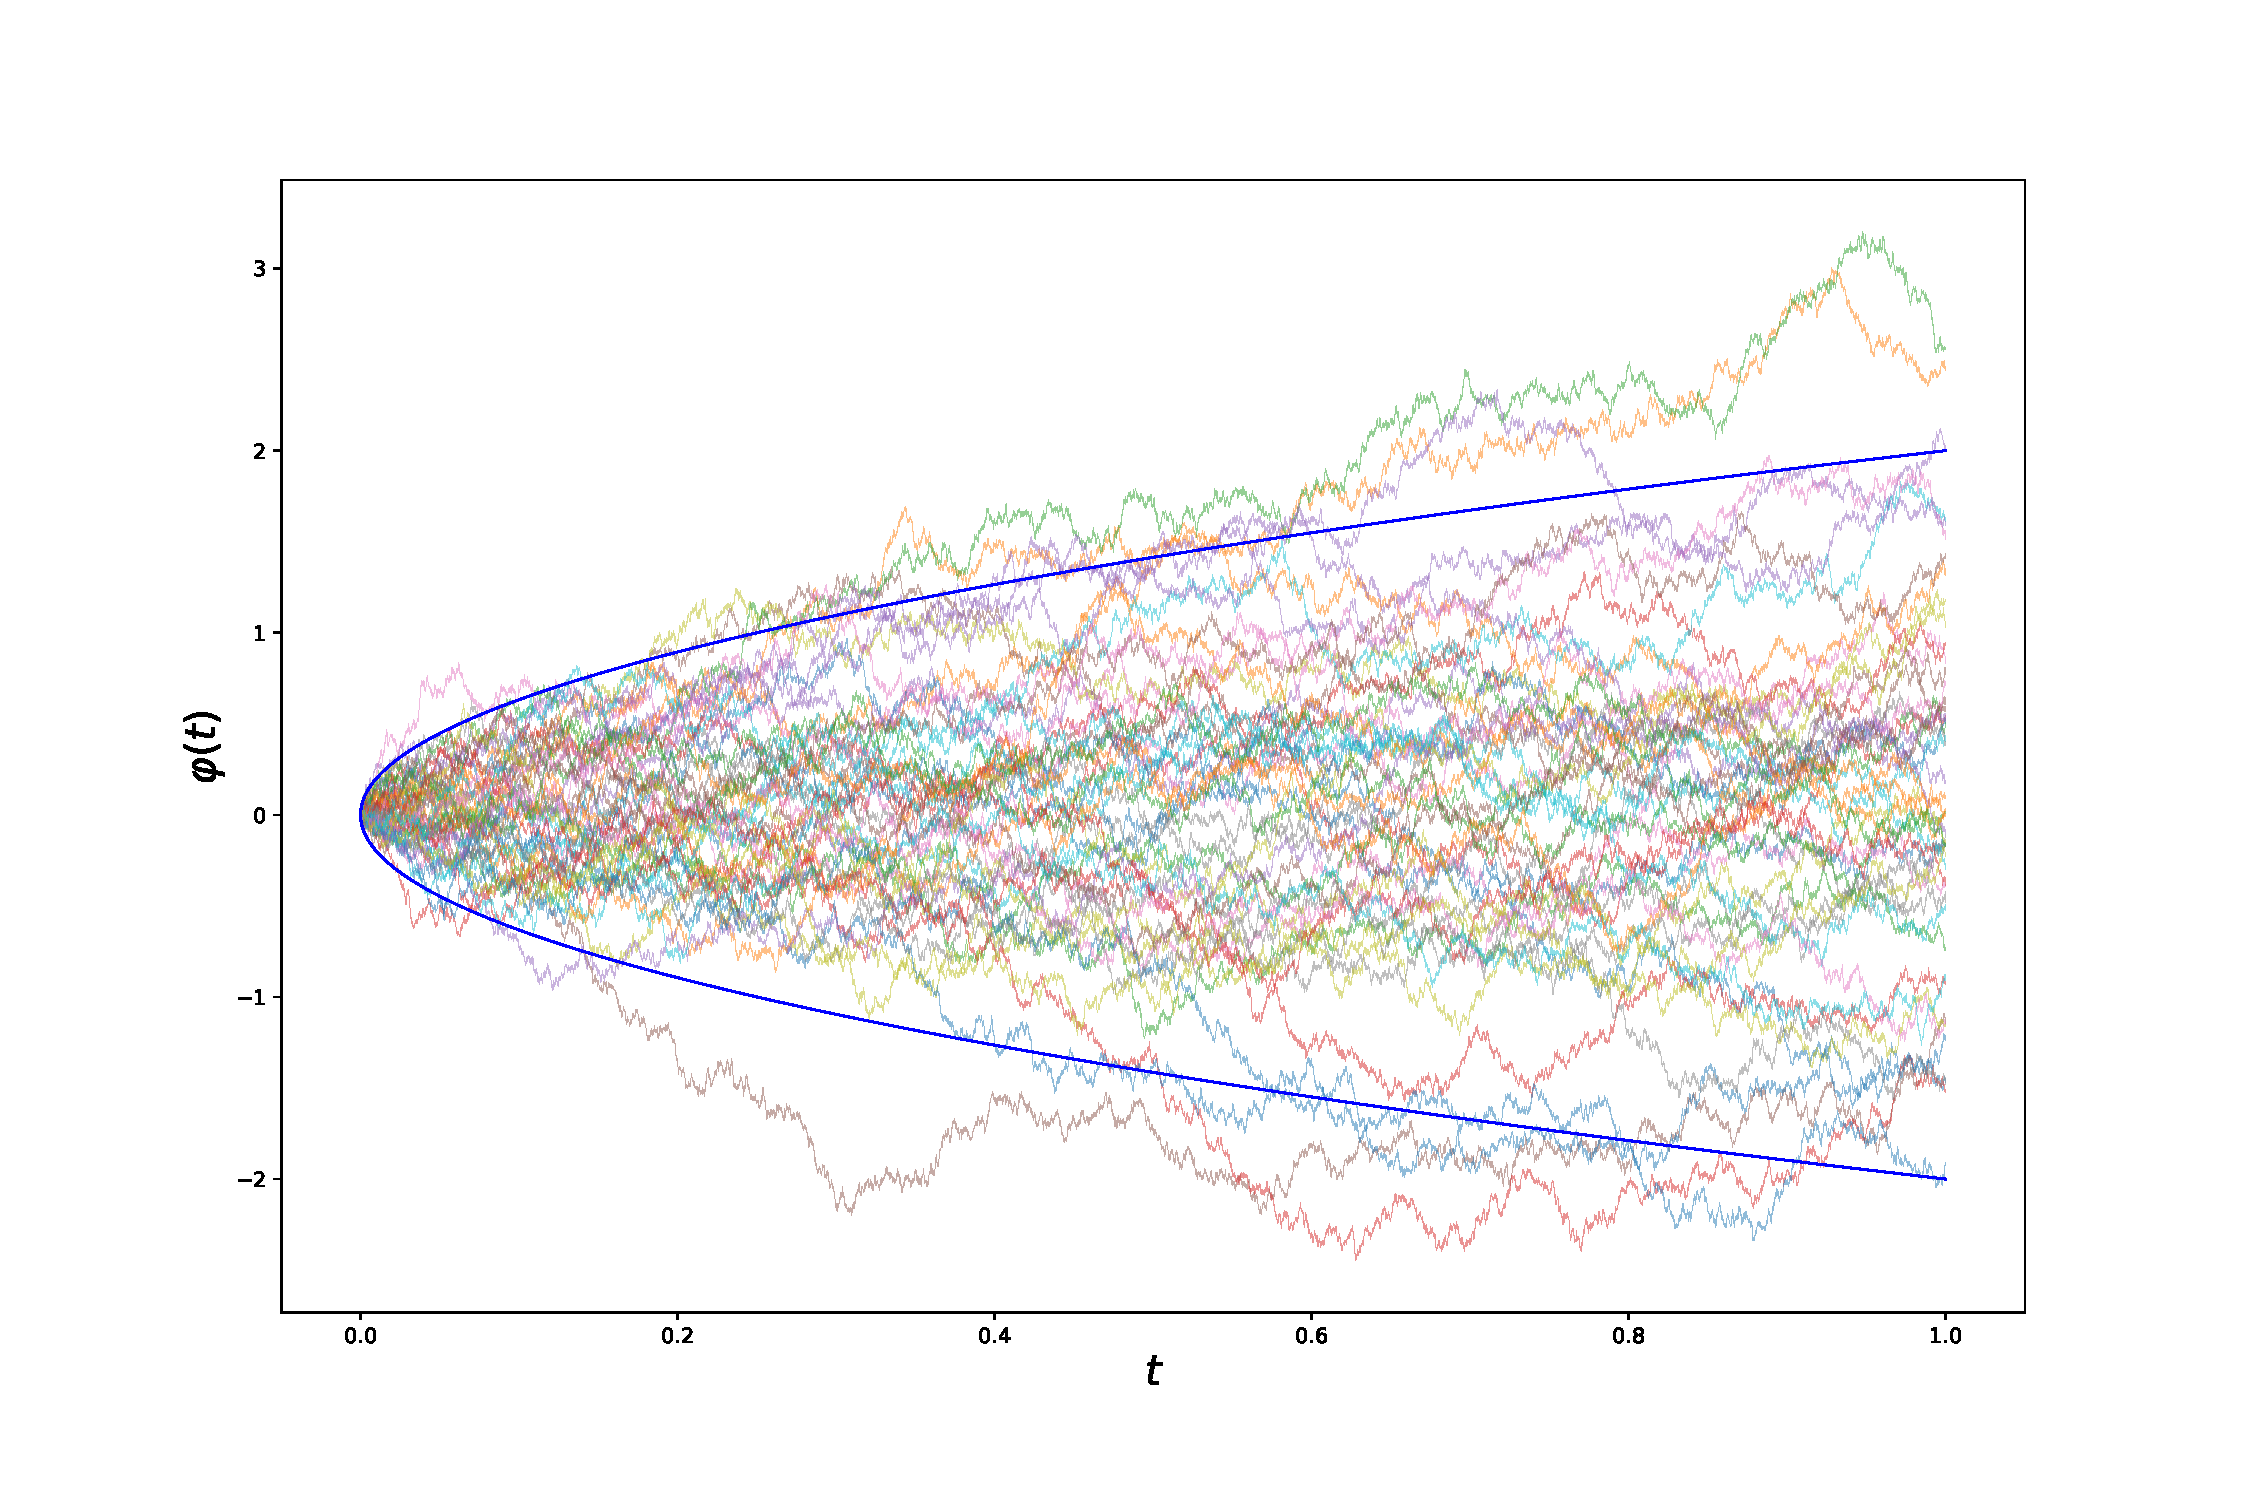
\includegraphics[width=0.9\textwidth]{images/bm.pdf}	
	\caption{Sample Paths of a Brownian Motion}
\end{figure}

Although it is computationally impossible to properly simulate a Brownian Motion, it can be approximated via the scaled random walk for big $n$. Figure \ref{fig:Brownian_Motion} shows this idea approximating a brownian motion with $n=9000$. In pursuance of pricing a European call option, we will see that it is possible to arrive at a closed form solution for these types of option. Nevertheless, more complex products may or may not have a closed form solution\\

To further develop the properties of the Brownian Motion, let us define the following:
\begin{definition}\label{def:quadratic_variation}
	Let $f$ be a real-valued function defined over $[0, T]$. Consider a partition $\Pi= \{t_i\}_{i=0}^{n}$ over $[0, T]$ where $t_0 = 0$, $t_n = T$, and $||\Pi|| = \max_j\{t_{j+1} - t_j\}$. We define the \textbf{Quadratic Variation} of $f$ up to time $T$ as
	\[
		[f, f]_T := \lim_{||\Pi|| \to 0} \sum_{t=0}^{n-1}\left[f(t_{j+1}) - f(t_{j})\right]^2
	\]
\end{definition}


The quadratic variation for a function $f$ represents the amount of total quadratic oscillation inside $D = [0,T]$. It can be shown (see \aycite{shreve}) that for $f \in C^1(D)$, $[f,f]_T = 0$.\\

%TODO: Is it relevant to prove this?
Asking how much does $W(t)$ oscillates between $D$ posses the question of whether $W(t) \in C^1(D)$. The answer is no, since the Brownian Motion is a continuous, nowhere-differentiable function. A consequence of this last remark is the following.

\begin{theorem}\label{th:quadratic_brownian_motion}
	Let $W(t)$ be a Standard Brownian Motion, then $[W, W]_T = T \ \forall \ T \geq 0$ almost surely.
\end{theorem}

\begin{proof}
	Let $\Pi = \{t_j\}_{j=0}^n$ be a partition of $[0, T]$. Define the sample quadratic variation corresponding to this partition to be
	
	\[
		Q_{\Pi} = \sum_{j=0}^{n-1}(W_{t_{j+1}} - W_{t_{j}})^2
	\]
	
	To show that $[W, W]_T = T$, is equivalent to show that, as $n\to\infty$, $\mathbb{E}[Q_\Pi] = T$ and $\mathbb{V}(Q_\Pi) = 0$ almost surely.\\
	
	First note that, by definition of the Standard Brownian Motion,
	\begin{equation}\label{eq:exp_change_bm}
		\mathbb{E}[(W_{t_{j+1}} - W_{t_{j}})^2] = \mathbb{V}[W_{t_{j+1}} - W_{t_{j}}] = t_{j+1} - t_{j}
	\end{equation}
	
	\begin{equation}\label{eq:var_change_bm}
		\mathbb{V}([W_{t_{j+1}} - W_{t_{j}}]^2) = 2(t_{j+1} - t_{j})^2
	\end{equation}
	
	Refer to appendix \ref{proof:var_change_bm} for a derivation of eq. \ref{eq:var_change_bm}.\\
	
	Consider now
	\begin{align*}
		\mathbb{E}[Q_\Pi] &= \mathbb{E}[\sum_{j=0}^{n-1}(W_{t_{j+1}} - W_{t_{j})}^2] \\
		&= \sum_{j=0}^{n-1}\mathbb{E}[(W_{t_{j+1}} - W_{t_{j}})^2] \\
		&= \sum_{j=0}^{n-1}(t_{j+1} - t_{j}) \\
		&= T
	\end{align*}
	
	Now,
	\begin{align*}
		\mathbb{V}(Q_T) &= \mathbb{V}(\sum_{j=0}^{n-1}(W_{t_{j+1}} - W_{t_{j}})^2) \shortintertext{By independence,}
		&=  \sum_{j=0}^{n-1}\mathbb{V}((W_{t_{j+1}} - W_{t_{j}})^2)\\
		&= \sum_{j=0}^{n-1} 2(t_{j+1} - t_{j})^2 \\
		&\leq 2 \sum_{j=0}^{n-1}||\Pi||\cdot (t_{j+1} - t_{j}) \numberthis
	\end{align*}
	
	Finally, note that
	
	\begin{equation}
		\lim_{||\Pi||\to 0} 2 \sum_{j=0}^{n-1}||\Pi||\cdot (t_{j+1} - t_{j}) = \lim_{||\Pi||\to 0} 2 ||\Pi|| T = 0
	\end{equation}
	$\therefore \lim_{||\Pi||\to 0} Q_\Pi = T$ almost surely.
\end{proof}

We state theorem \ref{th:quadratic_brownian_motion} informally by writing
\begin{equation}
	dW^2 = dt
\end{equation}

Two final consequences of \ref{th:quadratic_brownian_motion} are the following
\begin{equation}\label{eq:wt_0}
	\lim_{||\Pi||\to 0} \sum_{j=0}^{n-1}(W_{t_{j+1}} - W_{t_{j}})(t_{j+1} - t_{j}) = 0
\end{equation}

\begin{equation}\label{eq:w2_0}
	\lim_{||\Pi||\to 0} \sum_{j=0}^{n-1}(t_{j+1} - t_{j})^2 = 0
\end{equation}

Equations \ref{eq:wt_0} and \ref{eq:w2_0} are informally expressed as $dW_tdt = 0$ and $dt^2 = 0$

\chapter{A Primer on Option Pricing}
\chapter{Stochastic Calculus}
\chapter{The Black-Scholes-Merton Formula}
\chapter{Pricing Under Real Market Conditions}

\begin{appendices}
\addtocontents{toc}{\protect\setcounter{tocdepth}{1}}
\makeatletter
\addtocontents{toc}{%
  \begingroup
  \let\protect\l@chapter\protect\l@section
  \let\protect\l@section\protect\l@subsection
}
\makeatother
  \chapter{Aditional Proofs}
  \section{MGF for the symmetric random walk} \label{proof:mgf_srm}
  \begin{proposition}
  	The moment generating function of an scaled random walk $W^n(t)$ is $\varphi_{W^n}(u) = (\frac{1}{2}e^{\frac{u}{\sqrt{n}}} + \frac{1}{2}e^{-\frac{u}{\sqrt{n}}})^{nt}$
  \end{proposition}
  
  \begin{proof}
  By definition, the moment generating function for a scaled random walk is
  \begin{align*}
  	\mathbb{E}[e^{uW^n(t)}] &= \mathbb{E}(e^{\frac{u}{\sqrt{n}}M_{nt}})\\
  	&= \mathbb{E}\left[\exp\left(\frac{u}{\sqrt{n}}\sum_{k=0}^{nt}X_k\right)\right]\\
  	\shortintertext{Since $X_i \perp X_j \ \forall \ i \neq j$}
  	&= \prod_{k=1}^{nt}\mathbb{E}\left[\exp\left(\frac{u}{\sqrt{n}}X_k\right)\right]\\
  	&= \left[\frac{1}{2}\exp\left(\frac{u}{\sqrt{n}}\cdot 1 \right) + \frac{1}{2}\exp\left(\frac{u}{\sqrt{n}}\cdot -1\right) \right]^{nt}\\
  \end{align*}
  \end{proof}
  
  \section{MGF for the the normal distribution} \label{proof:mgf_nd}
  \begin{proposition}
  	The moment generating function for a random variable $X \sim N(0, t)$ is $\varphi_x(u) = e^{\frac{1}{2}u^2t}$
  \end{proposition}
  
  \begin{proof}
  	Recall, for $X \sim N(0, t)$,
  	\[f_X(x) = \frac{1}{\sqrt{2\pi t}}e^{-\frac{x^2}{2t}} \]  	
  	\begin{align*}
  	\shortintertext{Now,}
  		\mathbb{E}[e^{ux}] &= \int_{-\infty}^{\infty} e^{ux} f(x) dx \\
  		&= \frac{1}{\sqrt{2\pi t}}e^{ux - \frac{x^2}{2t}} \numberthis \label{mgf_eq1} \\
  	\end{align*}
  	\begin{align*}
	  	\shortintertext{Note that}
  		ux - \frac{x^2}{2t} &= \frac{2utx 	- x^2}{2t}\\
  		&= \frac{-1}{2t}\left[x^2 -2(ut)x + (ut)^2 - (ut)^2\right]\\
  		&= \frac{-1}{2t}\left[x - ut\right]^2 + \frac{1}{2}u^2t
  	\end{align*}
  	Thus, \ref{mgf_eq1} becomes
  	\begin{equation}
  		e^{\frac{1}{2}u^2t} \frac{1}{\sqrt{2\pi t}}\int_{-\infty}^{\infty}e^{-\frac{\left(x - ut\right)^2}{2t}} = e^{\frac{1}{2}u^2t}
  	\end{equation}
  \end{proof}
  
  \section{Derivation of equation \ref{eq:var_change_bm}} \label{proof:var_change_bm}
  \begin{proposition}
  Let $W_t$ be a standard Brownian Motion, 
  \begin{equation*}
  	\mathbb{V}(\left[W_{t_j+1} - W_{t_j}\right]^2) = 2\left(t_{j+1} - t_j\right)^2 \ \forall \ j \geq 0 
  \end{equation*}
  
  \begin{proof}
  \begin{align*}
  	\mathbb{V}(\left[W_{t_j+1} - W_{t_j}\right]^2) &= \mathbb{E}\left[\left(W_{t_j+1} - W_{t_j}\right)^2 - \mathbb{E}\left[W_{t_j+1} - W_{t_j}\right]^2\right] \\
  	&= \mathbb{E}\left[\left(W_{t_j+1} - W_{t_j}\right)^2 -\left(t_{j+1} - t_j\right)\right]^2 \\
  	&= \mathbb{E}\left[\left(W_{t_j+1} - W_{t_j}\right)^4  - 2\left(W_{t_j+1} - W_{t_j}\right)^2 \left(t_{j+1} - t_j\right) + \left(t_{j+1} - t_j\right)^2\right] \\
  	\intertext{Where $\mathbb{E}\left[\left(W_{t_j+1} - W_{t_j}\right)^4\right] = 3(t_{j+1} - t_j)^2$}
   	&= 2(t_{j+1} - t_j)^2
  \end{align*}
  \end{proof}
  \end{proposition}
  

\addtocontents{toc}{\endgroup}
\end{appendices}

\newpage
\nocite{*}
\bibliography{ref}
\end{document}